\documentclass[11pt,a4paper]{article}

\usepackage[margin=2.2cm]{geometry}
\usepackage[T1]{fontenc}
\usepackage{lmodern}
\usepackage{microtype}
\usepackage{amsmath}
\usepackage{booktabs}
\usepackage{tabularx}
\usepackage{longtable}
\usepackage{array}
\usepackage{enumitem}
\usepackage{xcolor}
\usepackage{listings}
\usepackage{tikz}
\usetikzlibrary{arrows.meta,positioning,fit,shapes.misc}
\usepackage[colorlinks=true,linkcolor=blue!50!black,urlcolor=blue!50!black,citecolor=blue!50!black]{hyperref}

\setlist{itemsep=2pt,topsep=4pt}
\setlength{\emergencystretch}{3em}
\newcolumntype{L}{>{\raggedright\arraybackslash}X}
\newcommand{\code}[1]{\texttt{#1}}
\newcommand{\file}[1]{\texttt{#1}}

\definecolor{codebg}{gray}{0.96}
\lstdefinelanguage{lean}{
  morekeywords={structure,def,theorem,example,where,fun,by,namespace,end,variable,
    import,open,deriving,if,then,else,match,with,intro,exact,obtain,unfold,cases,
    simp_all,omega,decide,grind,Prop,Type,True,False},
  sensitive=true,
  morecomment=[l]{--},
  morecomment=[s]{/-}{-/},
  morestring=[b]"
}
\lstset{
  basicstyle=\ttfamily\small,
  backgroundcolor=\color{codebg},
  keywordstyle=\color{blue!60!black}\bfseries,
  commentstyle=\color{green!40!black}\itshape,
  frame=single, rulecolor=\color{gray!40},
  breaklines=true, columns=fullflexible,
  xleftmargin=4pt, xrightmargin=4pt, aboveskip=6pt, belowskip=6pt
}

\title{\textbf{ContractForge}\\[4pt]
\large From English Requirements to Formally Verified Lean~4 Code with a Small Open-Weight Model\\[2pt]
\normalsize Design, Models, Architectural Decisions and Testing Strategy}
\author{AUTOSE-Leaniers}
\date{State as of 15 November 2026 (L0 v11, chain-v5)}

\begin{document}
\maketitle

\begin{abstract}
ContractForge is a multi-agent pipeline that turns a software requirements specification (SRS)
into Lean~4 code that is proved correct against a formal specification of each requirement.
Every layer is checked by Lean before the next one starts: a spec agent (L0) writes a
pre/post-condition contract per requirement, rule-based checks (L0.5) reject weak or broken
specs, an architect agent (L1) decomposes a spec into component contracts, and a coding agent
(L2) implements each component. The harness, not the model, writes and proves every proof
obligation, so a model cannot prove a weaker theorem under the right name. The pipeline runs
end to end with a local Qwen~2.5~7B model. On 18 SRS documents and 3 seeds, 400.7 of 517
specs (77.5\,\%) are verified end to end in the best setting, up from 343.3 of 483 (71\,\%) for
the previous harness. This document records what is implemented, which model and
infrastructure choices were made and why, the architectural decisions, and how the system is
tested and evaluated.
\end{abstract}

\tableofcontents
\newpage

%=====================================================================
\section{Goal and scope}
%=====================================================================

The goal is \emph{verified-by-construction} code from natural-language requirements. A
requirement is only considered implemented when Lean accepts, in one file, the spec, the
architecture, every implementation and a final theorem
\code{system\_ok : Spec.Satisfies (Impl)} derived from the framework's soundness theorem.

Design constraints that shaped every decision:
\begin{itemize}
  \item \textbf{Small open-weight model.} The main model is Qwen~2.5~7B Instruct, run locally.
        A 7B model makes syntax, API and reasoning mistakes that a large hosted model would
        not, so the harness is built to absorb them deterministically. Harness work that a
        small model would otherwise have to do is part of the method, not a shortcut.
  \item \textbf{SRS-independent fixes.} No fix may mention a field, function or requirement
        name of a particular SRS. Deterministic harness checks are preferred over prompt changes.
  \item \textbf{Lean core only.} No Mathlib, to keep builds and checks fast.
  \item \textbf{Reproducible, noise-aware evaluation.} Fixed seeds, three repetitions, and
        differences reported only when they exceed the seed spread.
\end{itemize}

The last intended step, turning verified Lean implementations into Python, is not built yet.

%=====================================================================
\section{System overview}
%=====================================================================

\begin{figure}[h]
\centering
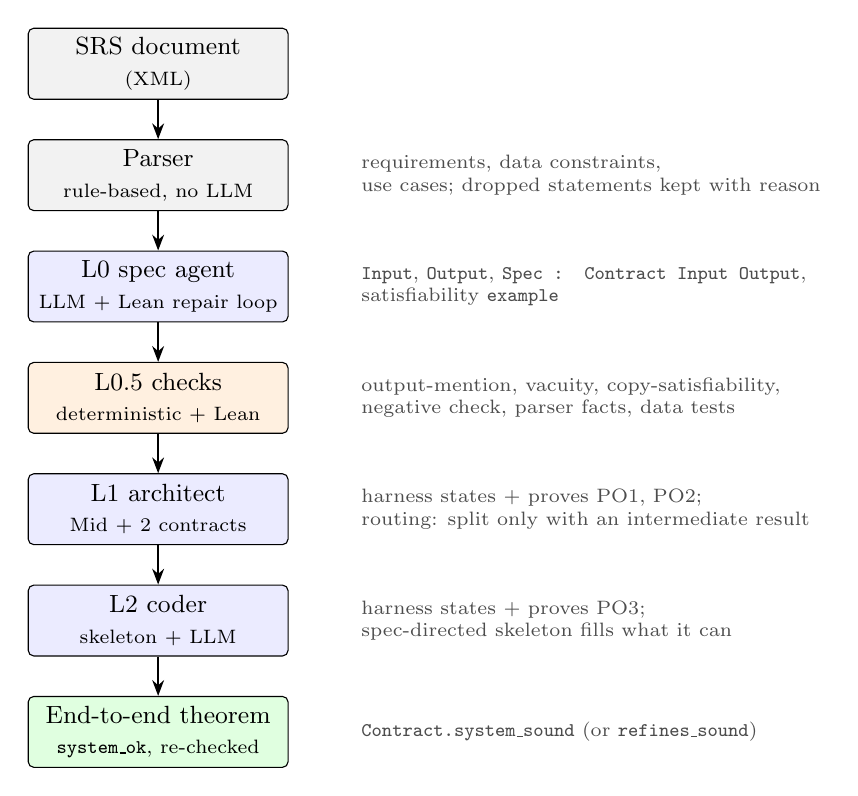
\begin{tikzpicture}[
  node distance=5mm and 6mm,
  box/.style={draw, rounded corners=2pt, align=center, minimum width=33mm, minimum height=9mm, font=\small, fill=#1},
  box/.default=white,
  arr/.style={-{Stealth[length=2mm]}, thick},
  note/.style={font=\scriptsize, align=left, text=black!70}
]
\node[box=gray!10] (srs) {SRS document\\\scriptsize (XML)};
\node[box=gray!10, below=of srs] (parse) {Parser\\\scriptsize rule-based, no LLM};
\node[box=blue!8, below=of parse] (l0) {L0 spec agent\\\scriptsize LLM + Lean repair loop};
\node[box=orange!12, below=of l0] (l05) {L0.5 checks\\\scriptsize deterministic + Lean};
\node[box=blue!8, below=of l05] (l1) {L1 architect\\\scriptsize Mid + 2 contracts};
\node[box=blue!8, below=of l1] (l2) {L2 coder\\\scriptsize skeleton + LLM};
\node[box=green!12, below=of l2] (end) {End-to-end theorem\\\scriptsize \code{system\_ok}, re-checked};

\foreach \a/\b in {srs/parse,parse/l0,l0/l05,l05/l1,l1/l2,l2/end} \draw[arr] (\a) -- (\b);

\node[note, right=8mm of parse] {requirements, data constraints,\\use cases; dropped statements kept with reason};
\node[note, right=8mm of l0] {\code{Input}, \code{Output}, \code{Spec : Contract Input Output},\\satisfiability \code{example}};
\node[note, right=8mm of l05] {output-mention, vacuity, copy-satisfiability,\\negative check, parser facts, data tests};
\node[note, right=8mm of l1] {harness states + proves PO1, PO2;\\routing: split only with an intermediate result};
\node[note, right=8mm of l2] {harness states + proves PO3;\\spec-directed skeleton fills what it can};
\node[note, right=8mm of end] {\code{Contract.system\_sound} (or \code{refines\_sound})};
\end{tikzpicture}
\caption{The ContractForge pipeline (per-spec ``chain'' path). Blue stages call the model; all
other stages are deterministic.}
\label{fig:pipeline}
\end{figure}

There are two L1/L2 paths:
\begin{description}
  \item[Chain path] (\code{main.py --until chain}): L1/L2 per spec. This is the path that is
        evaluated end to end and the subject of the results in Section~\ref{sec:results}.
  \item[Graph path] (\code{--until graph}, \code{--until arch}, \code{--until code}): a
        deterministic requirements graph groups L0 specs into components of a larger system;
        the model writes per-operation contracts over a harness-generated message type.
\end{description}

\paragraph{Division of labour.} The model writes \emph{definitions only}: L0 specs, L1
\code{structure Mid} and two contracts, L2 a function with the signature it is given. The
harness writes every proof-obligation statement, proves it with its own tactics, and when a
proof fails names the conjunct that does not follow.

%=====================================================================
\section{Formal foundation: the Lean framework}
%=====================================================================

The library \file{framework/ContractForge} (Lean 4.29.1, core only) defines assume/guarantee
contracts, the three proof obligations, sequential composition and the soundness theorems.

\begin{lstlisting}[language=lean]
structure Contract (A B : Type) where
  pre  : A -> Prop
  post : A -> B -> Prop

-- PO3: implementation f meets contract c
def Satisfies (c : Contract A B) (f : A -> B) : Prop :=
  forall x, c.pre x -> c.post x (f x)
-- PO1: c1's guarantee establishes c2's assumption
def Compatible (c1 : Contract A B) (c2 : Contract B C) : Prop :=
  forall x y, c1.pre x -> c1.post x y -> c2.pre y
-- PO2: c refines spec s
def Refines (c s : Contract A B) : Prop :=
  (forall x, s.pre x -> c.pre x) /\ (forall x y, s.pre x -> c.post x y -> s.post x y)
-- sequential composition
def seq (c1 : Contract A B) (c2 : Contract B C) : Contract A C where
  pre x    := c1.pre x
  post x z := exists y, c1.post x y /\ c2.post y z

theorem system_sound (h12 : Compatible c1 c2) (hr : (c1.seq c2).Refines s)
    (hf : c1.Satisfies f) (hg : c2.Satisfies g) : s.Satisfies (g . f)
\end{lstlisting}

\begin{table}[h]
\centering
\small
\begin{tabularx}{\linewidth}{l >{\raggedright\arraybackslash}p{0.3\linewidth} L l}
\toprule
PO & Lean & Meaning & Proved in \\
\midrule
PO1 & \code{Compatible c1 c2} & first guarantee establishes second assumption & L1 \\
PO2 & \code{Refines (c1.seq c2) Spec} & the composition refines the spec & L1 \\
PO3 & \code{Satisfies c f} & implementation meets its contract & L2 \\
\bottomrule
\end{tabularx}
\caption{Proof obligations. \code{system\_sound} combines them into end-to-end correctness.}
\end{table}

Other modules:
\begin{itemize}
  \item \file{Soundness.lean}: \code{seq\_sound}, \code{refines\_sound} (single component),
        \code{system\_sound}.
  \item \file{Chain.lean}: \code{compat\_seq}, \code{chain3\_sound} for chains of components (graph path).
  \item \file{Tactics.lean}: \code{discharge\_po [names]} (unfolds the named definitions, then
        \code{simp\_all}, \code{omega}, \code{grind}, \code{decide}); per-obligation tactics
        \code{discharge\_po1}, \code{discharge\_po2} (destructures the middle value of \code{seq}),
        \code{discharge\_po3} (splits an \code{if} in the implementation).
  \item \file{Strings.lean}: decidable string-format helpers over \code{List Char}
        (\code{allDigits}, \code{allAlnum}, \code{lenBetween}, \code{isMMYY}, \ldots), so data
        constraints can be stated and checked with \code{decide}.
\end{itemize}

%=====================================================================
\section{Models and infrastructure}
%=====================================================================

\subsection{Models}

\begin{table}[h]
\centering
\small
\begin{tabularx}{\linewidth}{>{\raggedright\arraybackslash}p{0.27\linewidth} >{\raggedright\arraybackslash}p{0.3\linewidth} L}
\toprule
Model & How it is run & Role \\
\midrule
\textbf{Qwen 2.5 7B Instruct} (Q4\_K\_M GGUF) & local \code{llama-server} (llama.cpp, CUDA) on port 8082, on a GPU node of the \emph{ada} cluster & \textbf{main model} for L0, L1, L2; all reported results \\
Gemma (\code{gemma-4-31b-it} / \code{26b-a4b-it}) & Google AI Studio API & early L0 spot checks; about 140\,s per call, so not used for full runs \\
DeepSeek (\code{deepseek-chat}) & API & supported provider, not used for reported results \\
Llama 3.3 70B & Groq API & supported provider, not used for reported results \\
\bottomrule
\end{tabularx}
\caption{Models supported by \file{harness/llm.py}. Model ids are overridable with
\code{CF\_*\_MODEL} environment variables.}
\end{table}

\paragraph{Why a local 7B model.} With a GPU it answers in seconds per entry, it is free to
rerun at scale (18 SRS $\times$ 3 seeds $\times$ several settings), it is reproducible with a
fixed seed, and it is the realistic target for a tool that should work without a paid API.
The cost is a weaker model, which the harness compensates for (Section~\ref{sec:decisions}).

\subsection{Generation settings}
\begin{itemize}
  \item Temperature 0.2 (\code{CF\_TEMPERATURE}); restart temperature 0.7 when the same error repeats.
  \item Seed 42 sent to the server; repetitions use seeds 42, 43, 44.
  \item Context 16\,384 tokens (8\,192 overflowed with repair history).
  \item Max output 2\,048 tokens, one retry at 4\,096; a truncated reply is never sent to Lean.
  \item Lean repair budget 5 attempts (\code{CF\_MAX\_RETRIES}); API errors (429/5xx/network) are
        retried separately, up to 6 times with exponential backoff.
\end{itemize}

\subsection{Compute and operations}
Runs are SLURM jobs on \emph{ada} (GTX 1080 Ti class GPUs). \file{main.py} starts and stops the
Qwen server itself. Lessons that are now encoded in the job files:
\begin{itemize}
  \item llama.cpp built with \code{-DGGML\_NATIVE=OFF} and explicit CUDA architectures, or it
        crashes on GPU nodes with an illegal-instruction error.
  \item Server readiness is checked with \code{curl -sf} (a loading server returns 503).
  \item Jobs request 32\,GB RAM (a 16\,GB job was OOM-killed mid-run) and exit at startup when
        the server has no usable GPU (a node with a broken CUDA ran Qwen on CPU at 4 tokens/s).
  \item \file{scripts/usage\_guard.sh} stops a run above 75\,\% GPU memory or job RAM.
\end{itemize}

%=====================================================================
\section{Architecture, stage by stage}
%=====================================================================

\subsection{Parser (\file{req\_parser.py})}
Rule-based and deliberately AI-free: the same XML bytes always give the same JSON bytes
(tested across hash seeds). It extracts requirements, data-dictionary constraints and use
cases, and drops statements that cannot become a Lean proposition (vague wording, UI steps,
technology choices, scope prose). Every dropped statement is kept with the rule that removed
it. It also records facts later used as checks: runtime bounds, length/charset/format rules
for data fields, and whether the requirement states a precondition.

\subsection{L0: spec agent (\file{agents/spec\_agent.py}, \file{agents/base.py})}
One prompt per entry; the model returns \code{structure Input}, \code{structure Output},
\code{def Spec : Contract Input Output} and an \code{example} proving
\code{Spec.pre i /\textbackslash{} Spec.post i o} by \code{decide}. The
\emph{generate~$\to$~check~$\to$~repair} loop (\code{generate\_verified}) is shared by all agents:
\begin{enumerate}
  \item \textbf{Extraction and fixups}: last Lean block that defines \code{Spec}; mechanical
        rewrites (\code{//} comments, \code{s.all} on strings, missing \code{deriving}).
  \item \textbf{Weakening guard}: a repair that makes \code{pre}/\code{post} weaker than the first
        attempt is rejected.
  \item \textbf{Lean check}: \code{lean\_runner.check\_lean}; \code{sorry} counts as failure.
  \item \textbf{Staged feedback} (\file{agents/repair.py}): only the earliest error layer
        (syntax $\to$ names $\to$ types $\to$ proof), first 3 errors with the offending line and a
        targeted hint; ``did you mean'' from Lean's own name list; Lean doc lookup
        (\file{lean\_docs.py}) quoting real signatures and docstrings of Lean 4.29.1.
  \item \textbf{Example-only repair}: when only the \code{example} is wrong the definitions are
        locked; the harness first searches for witness values itself.
  \item \textbf{Loop control}: same failure again $\to$ fresh prompt, then fresh prompt with a
        strategy hint, then stop. The attempt that got furthest is returned, not the last.
\end{enumerate}

\subsection{L0.5: spec checks (\file{validate.py}, \file{spec\_checks.py}, \file{agents/negative.py})}
Applied inside the loop (fed back to the model) and again on the final spec (report and
\file{review.json}):
\begin{itemize}
  \item housekeeping (one \code{Spec}, no \code{sorry}/\code{axiom}/\code{native\_decide}, has an example);
  \item contradictions (\code{x + n = x}) and consistent example inputs;
  \item parser facts (runtime bounds present) and data tests (valid and invalid sample strings
        from the parser's rules must be accepted and rejected);
  \item \textbf{vacuity}: changing each output field of the example must make \code{post} false
        for at least one change;
  \item \textbf{negative check}: the model names an input and an output the requirement
        \emph{forbids}; the harness writes the statement and Lean must prove
        \code{pre IN /\textbackslash{} \textasciitilde{} post IN OUT} (for data constraints, the
        forbidden inputs come from the parser, no LLM);
  \item \textbf{output-mention} (v11): every \code{post} conjunct must constrain the output, also
        after substituting outputs that \code{post} fixes elsewhere; otherwise it belongs in \code{pre};
  \item \textbf{copy-satisfiability} (v11): up to 48 implementations made only of copied input
        fields and constants are tried against \code{Spec} in one Lean run. A hit marks the spec
        \emph{weak}; it is fed back once, then accepted and recorded (strong / weak / copy-ok).
\end{itemize}
\code{--on-l0-fail stop|redo|exclude|loop} decides what happens to entries that still fail.

\subsection{Chain path: L1 and L2 per spec (\file{chain\_pipeline.py})}

\paragraph{Routing.} A spec is split into two components only if a \code{post} condition
relates two output fields (an \emph{intermediate result}, e.g.\ a message defined in terms of
the result list). Everything else is verified as one component: its architecture is
\code{Spec} itself and PO2 is \code{Refines Spec Spec}, with no model call.

\paragraph{L1 architect (\file{agents/chain\_architect.py}, \file{chain\_checks.py}).} The
model writes \code{structure Mid} and contracts \code{A : Input $\to$ Mid},
\code{B : Mid $\to$ Output}. Checks before and in Lean:
\begin{itemize}
  \item shape and \textbf{visibility}; since chain-v5 the harness itself carries every
        \code{Input} field the second contract reads into \code{Mid};
  \item \textbf{work}: identity splits, copies of \code{Spec} up to renaming, and a second
        contract that ignores the first's result are rejected; two identity splits make the
        spec ``not decomposable'' and it is verified as one component;
  \item \textbf{constant result}: the first component is rejected if every result field is
        provably constant or a disguised copy of an input field;
  \item \textbf{PO1 with repair}: conjuncts of the second \code{pre} that the first \code{post}
        does not give are removed by the harness (sound, since PO2 does not use the second
        \code{pre}); then PO1 and PO2 are proved by \code{discharge\_po1/2};
  \item a strength record (out of 6) for every accepted architecture.
\end{itemize}

\paragraph{L2 coder (\file{agents/chain\_coder.py}, \file{skeleton.py}).} For each contract the
harness first derives a \textbf{spec-directed skeleton} from \code{post}:
\code{o.f = e} $\to$ \code{f := e}; \code{o.f = true $\leftrightarrow$ c} $\to$ \code{decide c};
\code{A $\to$ o.f = e} $\to$ \code{if}; \code{$\forall$ e $\in$ o.L, P e} $\to$ \code{filter}.
If the skeleton is complete, PO3 is attempted with no model call (\code{harness\_only});
otherwise the skeleton with \code{FILL} holes is put in the prompt. Record fields are compared
with the result structure before Lean, and PO3 failures are reported as the \code{post}
conjuncts the function does not establish, with suggested actions.

\paragraph{End.} One file per spec: spec, architecture, implementations and
\code{theorem system\_ok}, re-checked by Lean (\code{full\_check}).
\code{--fallback-single} implements \code{Spec} as one component when a split fails, reported
as its own mode.

\subsection{Graph path (\file{req\_graph.py}, \file{arch\_lean.py}, \file{agents/architect\_agent.py})}
A deterministic graph (spaCy lemmas, no LLM) links operations (one per compiling L0 spec)
through shared entities taken from the SRS (data dictionary, glossary, actors) and from the
specs themselves (helper structures; state fields one spec writes and another reads). Groups
are connected parts; components come from Louvain clustering (always above 8 operations, from 4
when modularity $\ge 0.1$). Cycles are broken, keeping the order with the least backward data
flow. The harness writes a message type, a locked \code{SystemSpec} (one \code{match} case per
L0 spec), and every trace/PO1/PO2/\code{system\_sound} statement; the model writes only
per-operation \code{pre}/\code{post}. An operation whose contract fails is \emph{degraded} to its
L0 conditions so the group can still be proved. This path is built and tested but has not been
the focus of recent runs.

%=====================================================================
\section{Key architectural decisions}
\label{sec:decisions}
%=====================================================================

\small
\begin{longtable}{>{\raggedright\arraybackslash}p{0.27\linewidth} >{\raggedright\arraybackslash}p{0.33\linewidth} >{\raggedright\arraybackslash}p{0.32\linewidth}}
\toprule
Decision & Why & Evidence / effect \\
\midrule
\endhead
Model writes definitions only; the harness writes and proves every PO statement &
A model could prove a weaker theorem under the right name; proofs by a 7B model were the main failure &
Replaying v2: the harness's tactics proved PO1/PO2 for all 38 accepted architectures and PO3 for all 64 accepted implementations. Proofs were never the bottleneck \\
Every layer checked by Lean before the next starts; verified code is locked context &
Errors must not propagate; later agents must not edit earlier results &
Locked context is prepended at check time; redeclarations are stripped \\
Rule-based, deterministic parser &
Reproducibility; every dropped statement is auditable &
Same bytes in, same bytes out (tested) \\
Staged, targeted repair feedback instead of raw Lean output &
A 7B model drowns in long error lists &
L0 compile rate 30/75 $\to$ 55/75 with prompt v2 + repair loop, later 67/74 \\
Lean doc lookup from the real Lean environment &
Qwen invents APIs (\code{List.nth}, \code{String.toInt}) &
In replay, 56 of 110 saved compile failures receive a relevant entry \\
Negative check and vacuity check &
``Compiles'' does not mean ``says enough'': a login spec accepted any password &
47 of 75 gamma j specs proven to reject a forbidden output (v8) \\
Output-mention and copy-satisfiability checks in L0 (v11) &
Specs whose \code{post} only constrains the input can never be implemented; weak specs verify with stubs &
Replay: 32 of 541 specs fail output-mention; 0 of the 30 that reached chain-v4 ever verified \\
Route to a split only on an intermediate result &
Forcing splits produced fake decompositions (copy fields + constant flag) &
chain-v3: 11 of 12 verified gamma j chains were fake; all rejected under v4 \\
Constant-result and identity checks in Lean &
The model satisfied textual identity checks with a constant field &
Strength score now requires the first result to depend on the input \\
Harness carries \code{Input} fields into \code{Mid}; PO1 repair &
Visibility and success-case \code{pre} were the main L1 failures &
7 of 8 L1 visibility failures fixed in replay \\
Spec-directed skeleton for L2 &
Much of an implementation follows mechanically from \code{post}; a small model should spend its effort on the rest &
Replay: skeleton alone proves PO3 for 751 of 1059 previously implemented components \\
Loop control: change strategy, stop early &
25 of 50 L1 failures repeated the same stage 5 times &
Fewer wasted attempts; loops stopped early are counted \\
Graph path: message type, not a shared \code{World} record &
A single \code{World $\to$ World} step cannot satisfy conflicting operations (login/logout) &
Agreed with the team \\
Graph path: degrade failing operations, break cycles &
One failing trace blocked the whole group; merging cycles put 47 of 52 operations in one component &
Replay: rejected groups become accepted-degraded, 98/98 obligations \\
Lean core only, no Mathlib; Lean 4.29.1 pinned &
Fast builds and checks; stable names for prompts & --- \\
Every fix SRS-independent with a \code{CF\_*} off-switch &
Avoid overfitting to the two development SRSs; allow ablations &
Each v11/chain-v5 fix can be disabled individually \\
\bottomrule
\end{longtable}
\normalsize

%=====================================================================
\section{Version history}
%=====================================================================

\small
\begin{longtable}{>{\raggedright\arraybackslash}p{0.12\linewidth} >{\raggedright\arraybackslash}p{0.12\linewidth} >{\raggedright\arraybackslash}p{0.68\linewidth}}
\toprule
Version & Date & Main change and result \\
\midrule
\endhead
L0 v1 & 2026-10-30 & Hardened prompt (no Lean~3 syntax, no redefinition of \code{Contract}, satisfiability example): 30/75 compile \\
L0 v2 & 2026-10-31 & Conversational repair loop, error-type hints, restart at higher temperature: 55/75 \\
L0 v3--v4 & 2026-10-31 & Staged repair, fixups, L0.5 checks, witness search, 16k context: 65/75 compile \\
L0 v5--v8 & 2026-10-31 & Negative check; harness bug fixes (\code{sorry} detection, best attempt, vacuity false alarm): 68/75 compile, L0.5 56 pass \\
L0 v9 & 2026-11-02 & Search/filter/sort prompt section and template; parser keeps filter/sort sentences \\
L0 v10.1 & 2026-11-02 & Seeds and repetitions, \file{Strings.lean}, name suggestions, truncation handling. Frozen as the L0 baseline: 67 compile, 61 L0.5 pass (gamma j, 3 seeds) \\
chain v1--v2 & 2026-11-06 & First L1/L2 end to end: v1 0/61; v2 19/61 gamma j (mostly identity splits) \\
chain-v3 & 2026-11-12 & Model writes definitions only; single-step routing; visibility and identity checks; failure classes; 38.67/61 gamma j \\
chain-v4 & 2026-11-13 & Routing by intermediate result, constant-result check, PO1 repair, weak-spec flag; extended to 18 SRS \\
L0 v11 + chain-v5 & 2026-11-13/14 & Output-mention and copy-satisfiability in L0, Lean doc lookup, \code{Mid} carrying, not-decomposable mode, spec-directed skeleton, loop control \\
\bottomrule
\end{longtable}
\normalsize

%=====================================================================
\section{Testing strategy}
%=====================================================================

Testing works at four levels: unit tests of the harness, Lean-only replays of stored model
output, controlled runs with the real model, and the evaluation protocol.

\subsection{Unit and regression tests}
\code{cd harness \&\& python -m pytest}: 194 tests, about 4 minutes with Lean. Tests that need
Lean are skipped when \code{lake} is missing; graph tests need spaCy and networkx. Every fixed
harness bug gets a regression test.

\begin{table}[h]
\centering
\small
\begin{tabularx}{\linewidth}{l r L}
\toprule
File & Tests & Covers \\
\midrule
\file{test\_req\_parser.py} & 6 & parser determinism across hash seeds, drop rules \\
\file{test\_harness\_fixes.py} & 28 & Lean extraction, locked-example repair, \code{sorry} detection, best-attempt selection, contradiction checks, fixups, repair hints \\
\file{test\_negative\_check.py} & 8 & negative check on real specs; unusable examples never block \\
\file{test\_v9\_fixes.py} & 6 & filter/sort parsing, scope drops, per-mutant vacuity, search template \\
\file{test\_v10\_fixes.py} & 29 & seeds and metadata, truncation, rule-based negatives, name suggestions, string helpers \\
\file{test\_v11\_fixes.py} & 28 & output-mention, copy-satisfiability, doc lookup, skeleton, loop control \\
\file{test\_l05\_loop.py} & 4 & L0.5 feedback loop \\
\file{test\_req\_graph.py} & 15 & graph determinism, edges, state entities, split rule, broken cycles \\
\file{test\_arch.py} & 15 & every L1 tool on a toy shop; correct and rejected architectures; degrading \\
\file{test\_chain.py} & 26 & static checks, routing, constant result, PO1 repair, PO diagnosis, pipeline with a scripted model, repetition summary \\
\file{test\_coder.py} & 14 & L2 coder, record-field feedback \\
\file{test\_code\_lean.py} & 15 & harness-written L2 Lean (graph path) \\
\midrule
Total & 194 & \\
\bottomrule
\end{tabularx}
\caption{Test suite by file.}
\end{table}

\subsection{Scripted and fake models}
Pipelines are tested end to end without an LLM: a scripted model returns fixed replies to
exercise every branch of the chain pipeline, and a ``copy the L0 spec'' fake model exercises
the graph L1 plumbing at full scale (113/113 obligations on the gamma j graph). These test the
plumbing only, not model behaviour.

\subsection{Lean-only replays of stored model output}
Before a new harness version is run with the model, it is replayed on every stored record of
the previous run (specs, architectures, implementations) with Lean only. This measures what a
check would have accepted or rejected and catches false alarms before GPU time is spent (for
example, the first output-mention check had 2 false alarms on specs that had verified, fixed
before the run). Prompt examples are themselves run through the static checks and Lean.

\subsection{Model runs and evaluation protocol}
\begin{itemize}
  \item \textbf{Repetitions}: every setting is run with seeds 42, 43, 44; results are
        reported as mean (min--max). Single runs moved by $\pm 5$ L0.5 passes on their own,
        so earlier single-run ``improvements'' were partly noise.
  \item \textbf{Spread rule}: \file{evaluation/compare\_runs.py} calls a difference better or
        worse only when $|\Delta\text{mean}|$ exceeds the spread of the runs.
  \item \textbf{Run metadata}: every run stores harness version, prompt hashes, git commit and
        dirty flag, model id, temperature, seed and the L0 run it read.
  \item \textbf{Frozen inputs}: L1/L2 read a frozen L0 run, so L1/L2 changes are compared on
        identical specs.
  \item \textbf{Ablation}: chain-v5 is also run on the old v10.1 L0, separating the L1/L2
        effect from the L0 effect.
  \item \textbf{Held-out SRS}: development used gamma j and video search; the 16 other SRS
        documents were not looked at when designing the fixes.
  \item \textbf{Failure classes}: every failure gets a class (shape, visibility, identity, po1,
        po2, po3, unknown-field, syntax, \ldots) and \file{summarize\_e2e.py} counts them per run.
\end{itemize}

\subsection{Metrics}
\begin{description}
  \item[End to end] the whole spec file, including \code{system\_ok}, is accepted by Lean.
  \item[Weak spec] Lean accepts an implementation made only of copied inputs and constants.
  \item[End to end, non-trivial] end to end on specs that are not weak; the main quality number.
  \item[Model wrote code] the verified implementation contains model-written code (not only the
        harness skeleton). Reported next to the total so the harness's share is visible.
  \item[Strength] for two-component architectures, a score out of 6 for real decomposition.
\end{description}

%=====================================================================
\section{Current results}
\label{sec:results}
%=====================================================================

All 18 SRS documents, Qwen 2.5 7B, seeds 42--44; sums over SRS of the per-SRS mean.
Non-trivial = specs not satisfiable by copies and constants.

\begin{table}[h]
\centering
\small
\begin{tabular}{l r r r r r}
\toprule
Run & Specs & End to end & Rate & Non-trivial e2e & Non-trivial rate \\
\midrule
chain-v4 strict (v10.1 L0) & 483 & 343.3 & 71.1\,\% & 149.7 & 58\,\% \\
chain-v4 fallback & 483 & 365.0 & 75.6\,\% & 157.3 & 61\,\% \\
chain-v5 strict on v10.1 L0 (ablation) & 483 & 372.0 & 77.0\,\% & 163.7 & 64\,\% \\
L0 v11 + chain-v5 strict & 517 & 390.3 & 75.5\,\% & 193.3 & 64\,\% \\
\textbf{L0 v11 + chain-v5 fallback} & 517 & \textbf{400.7} & \textbf{77.5\,\%} & \textbf{200.0} & \textbf{66\,\%} \\
\bottomrule
\end{tabular}
\caption{End-to-end verification. Of the 193.3 non-trivial strict results, 64.0 contain model-written code; the rest are completed by the harness skeleton.}
\end{table}

\paragraph{Reading.}
\begin{itemize}
  \item The L1/L2 changes (chain-v5) are a clear gain: on the same specs, 71\,\% $\to$ 77\,\%,
        better or equal on every SRS, beyond the seed spread on six.
  \item The new L0 (v11) produces 34 more specs but does not raise the pass \emph{rate}; the
        higher absolute count comes from chain-v5 and from more specs.
  \item \code{--fallback-single} is the best setting.
\end{itemize}

%=====================================================================
\section{Known limitations and next steps}
%=====================================================================
\begin{itemize}
  \item \textbf{L0 v11 regressions} on gamma j ($\approx 53 \to 49$), ertms ($31$--$33 \to 28$--$29$)
        and dii ($5 \to 3$), not seen in the ablation, so caused by L0 v11; failures are mostly PO3.
        Not yet investigated.
  \item Two SRS (peering, get real 0.2) parse to one requirement that is flagged at L0.5, so no
        spec reaches L1.
  \item Each chain repetition reads the same L0 run (\code{rep1}); the seed spread covers L1/L2
        only, not L0.
  \item Real two-component decompositions remain rare with a 7B model; most specs are single
        component by routing. The graph path is the place for system-level architecture.
  \item ``Checked'' and ``verified'' mean consistent with the spec, not that the spec matches
        the requirement; specs still need human review for meaning.
  \item Not built: Lean $\to$ Python translation, re-verification tool (\file{reverify.py}), a
        benchmark system beyond the gamma j gold L0.
\end{itemize}

\appendix
\section{Repository map}
\small
\begin{tabularx}{\linewidth}{l L}
\toprule
Path & Contents \\
\midrule
\file{framework/ContractForge/} & Lean library: \file{Contract}, \file{Soundness}, \file{Chain}, \file{Tactics}, \file{Strings} \\
\file{harness/main.py} & entry point: parse $\to$ spec $\to$ check $\to$ graph/arch/code or chain \\
\file{harness/agents/} & spec agent, architects, coders, shared repair loop, fixups, negative check \\
\file{harness/chain\_*.py}, \file{po.py}, \file{skeleton.py} & chain path: checks, failure classes, PO statements and proofs, L2 skeleton \\
\file{harness/validate.py}, \file{spec\_checks.py}, \file{lean\_docs.py} & L0.5 checks and Lean documentation lookup \\
\file{harness/req\_parser.py}, \file{req\_graph.py} & SRS parser; requirements graph \\
\file{evaluation/} & \file{compare\_runs.py}, \file{summarize\_e2e.py}, \file{summarize\_l05loop.py} \\
\file{runs/<doc>/<run>/rep<k>/} & per-run outputs: \file{specs.json}, \file{l1l2.json}, Lean files, \file{summary.md} \\
\file{MEMORY.md} & running log of decisions, results and next steps \\
\bottomrule
\end{tabularx}

\end{document}
